\documentclass[UTF8]{ctexart}

\usepackage[linesnumbered,boxed,ruled,commentsnumbered]{algorithm2e}
\usepackage{bm}
\usepackage{graphicx}
\usepackage{float}
\usepackage[bookmarks=true]{hyperref}
\usepackage{amsmath}
\begin{document}
\title{CompBio Homework2}
\author{陈昭熹 2017011552}
\maketitle
\tableofcontents
\newpage
\section{层次聚类}
数据经过预处理后(主要是将行列互换使得两个文件中的表头对齐),可以绘制出如下层次聚类结果。
\subsection{树状图}
\begin{figure}[H]
    \centering
    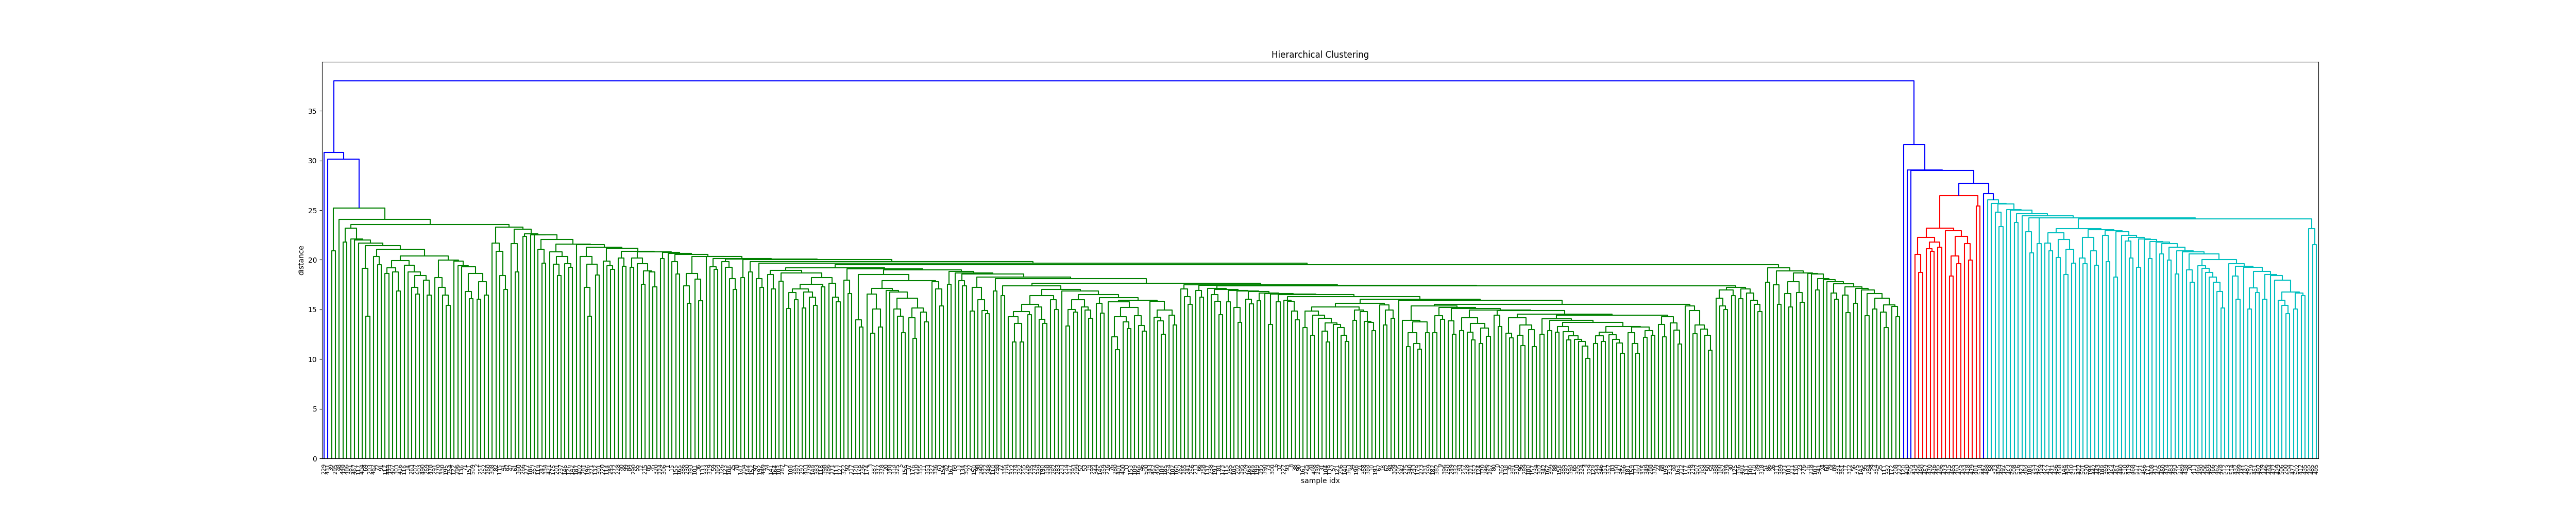
\includegraphics[scale=0.1]{../HClust.png}
\caption{Hierarchy Cluster}
\end{figure}

利用该树进行二分类,并使用$ER\_Status\_nature2012$作为分类标准,评估分类准确率为:
\begin{equation}
    Accuracy = 93.68\%
\end{equation}
\subsection{Heatmap}
利用seaborn库中的聚类方法,以Gene为横轴,Patients为纵轴绘制出Heatmap如下,可以看出,病人被明显的分为了两类,这为后面的分析提供了便利。
\begin{figure}[H]
    \centering
    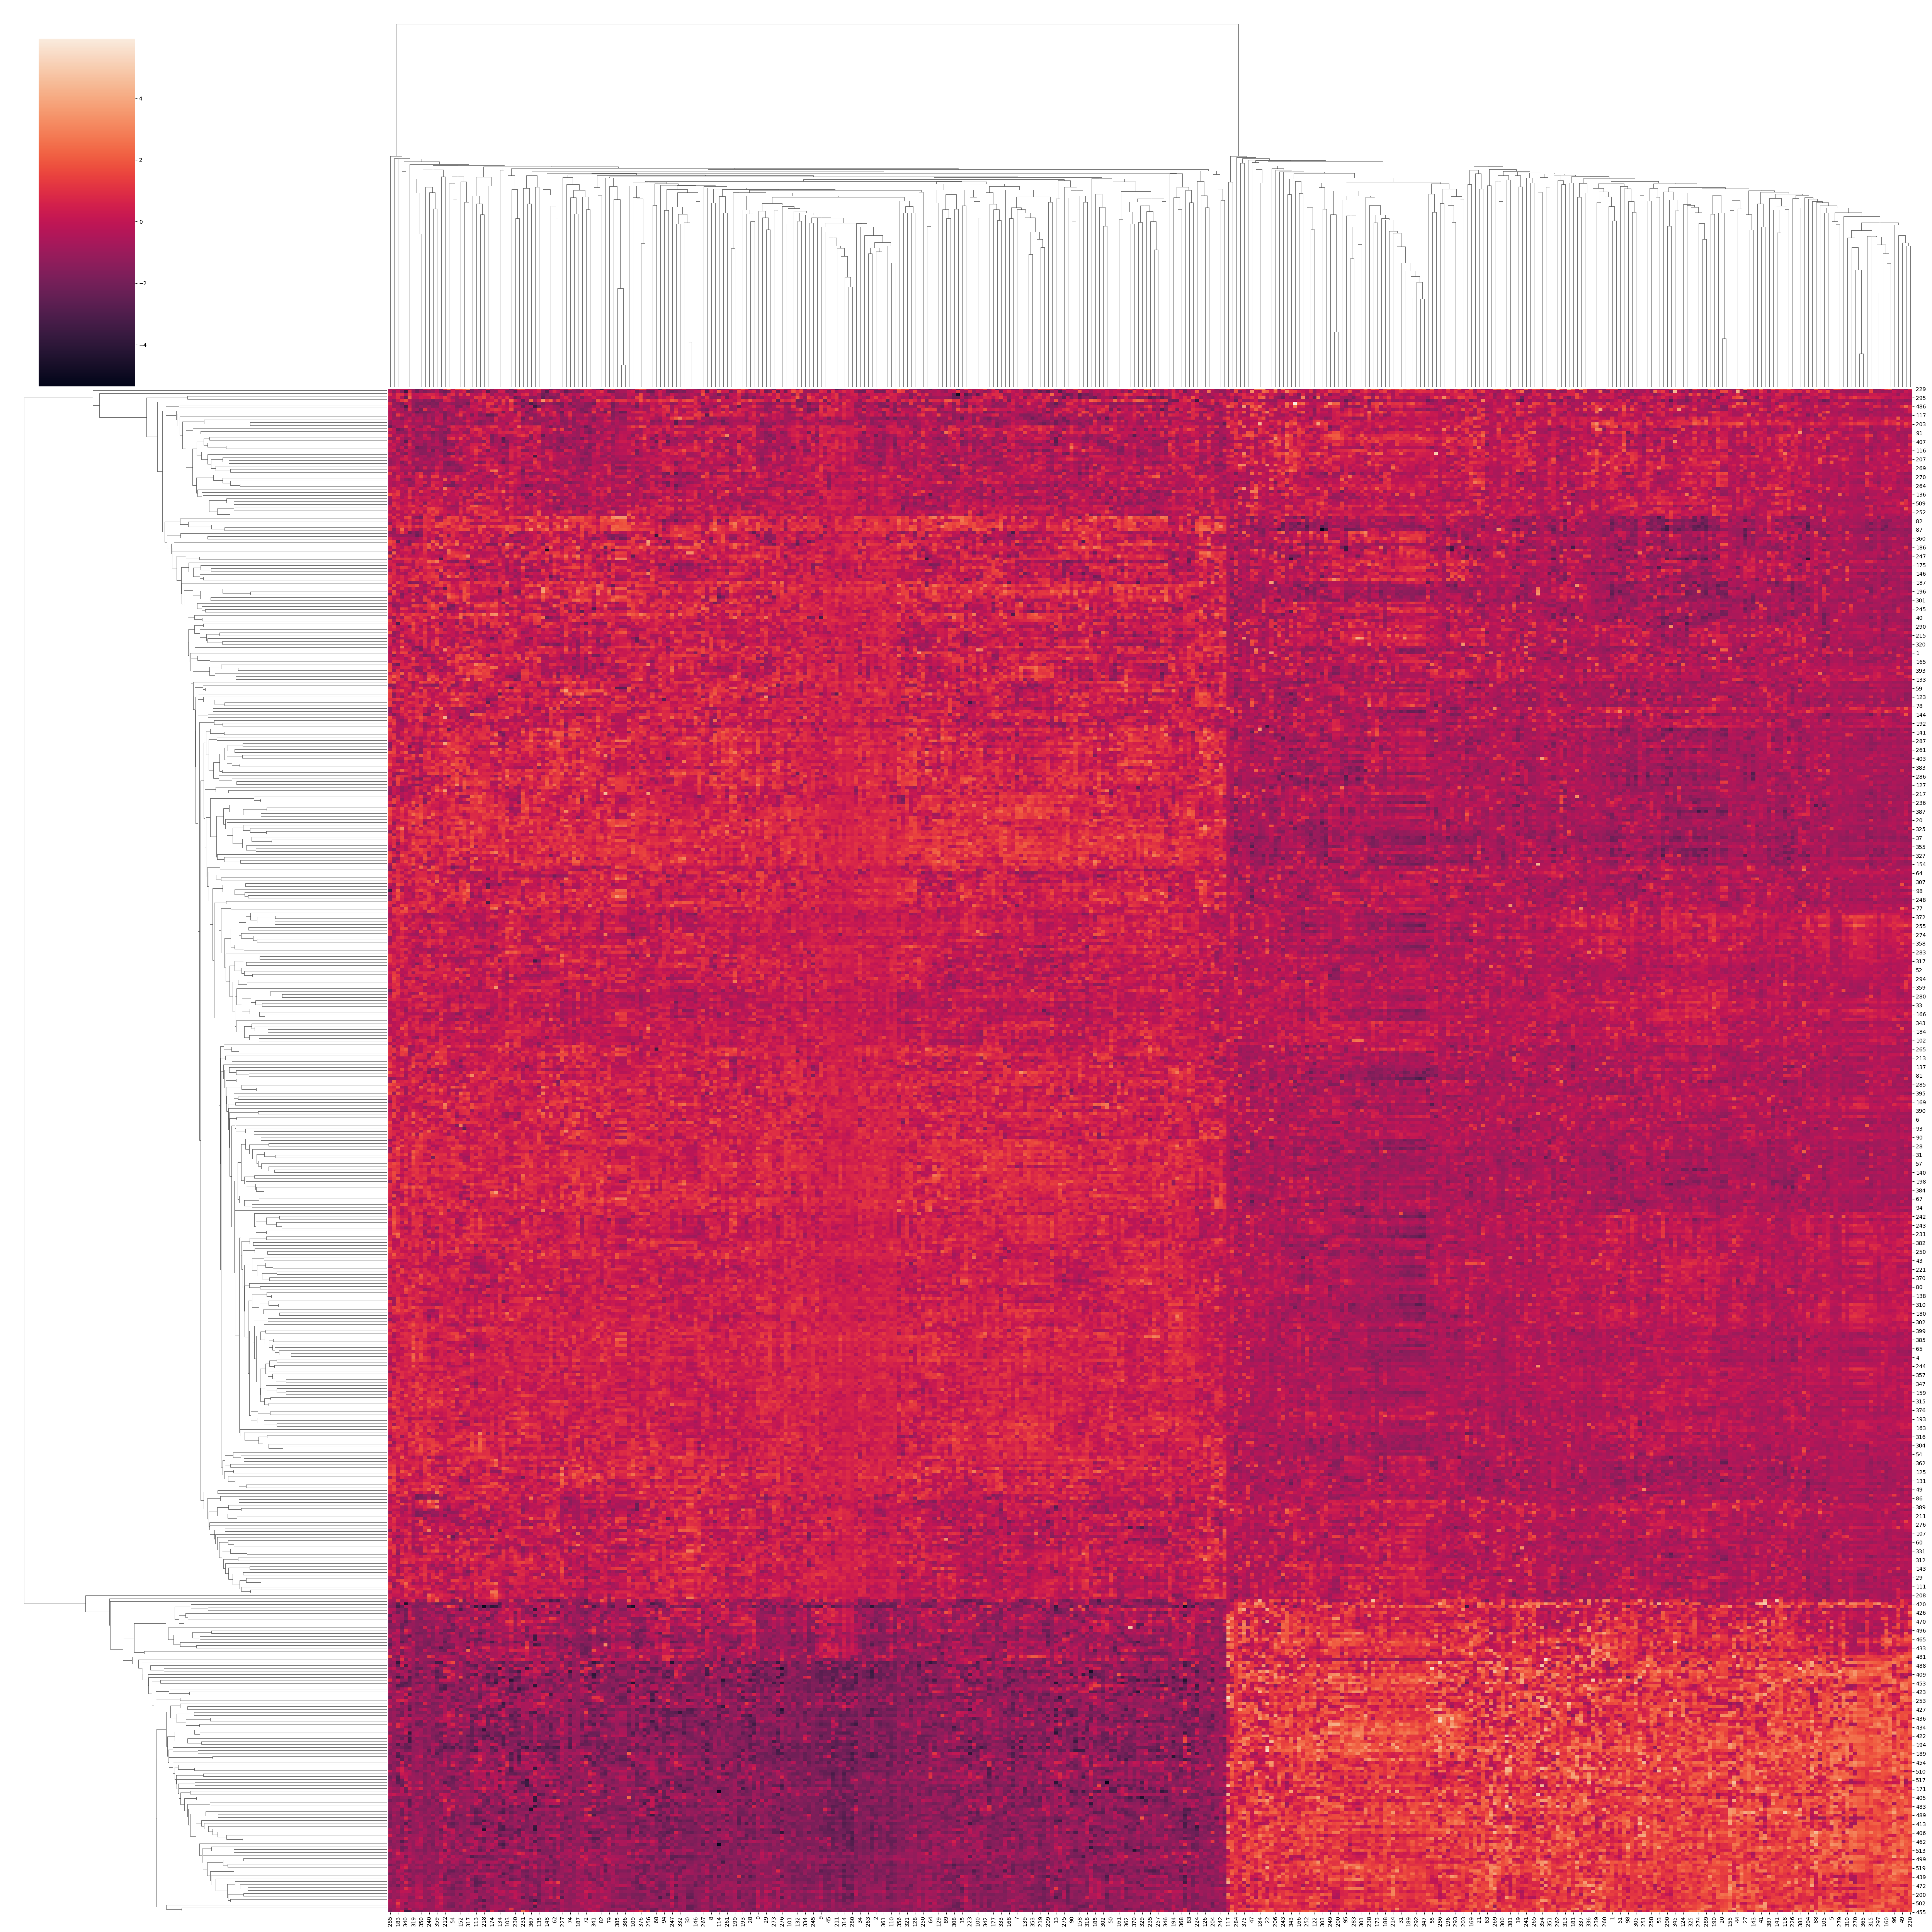
\includegraphics[scale=0.08]{../heatmap.png}
    \caption{HeatMap}
\end{figure}
\section{PCA降维}
\subsection{实现思路}
主要是依据PCA的数学原理进行实现,首先计算协方差阵,后计算协方差阵特征值和特征向量,并按照特征值从大到小排序,根据特征值大小选择主成分,从而确定变换矩阵。利用变换矩阵完成原始数据的降维。
\subsection{主成分选取依据}
在本次作业的数据中,使用上述方法后,输出前5个主成分所对应的特征值如下:
\begin{equation}
    [190.72474391,11.58899724,8.35373783,6.27501677,   5.33837007]
\end{equation}

可以看出第一个主成分远远超出后面的成分,代表着以第一个主成分为特征时就可以将数据较好的区分开,因此选取第一个主成分表示原数据特征,将原始数据降至一维。

\subsection{降维后聚类效果}
\begin{figure}[H]
    \centering
    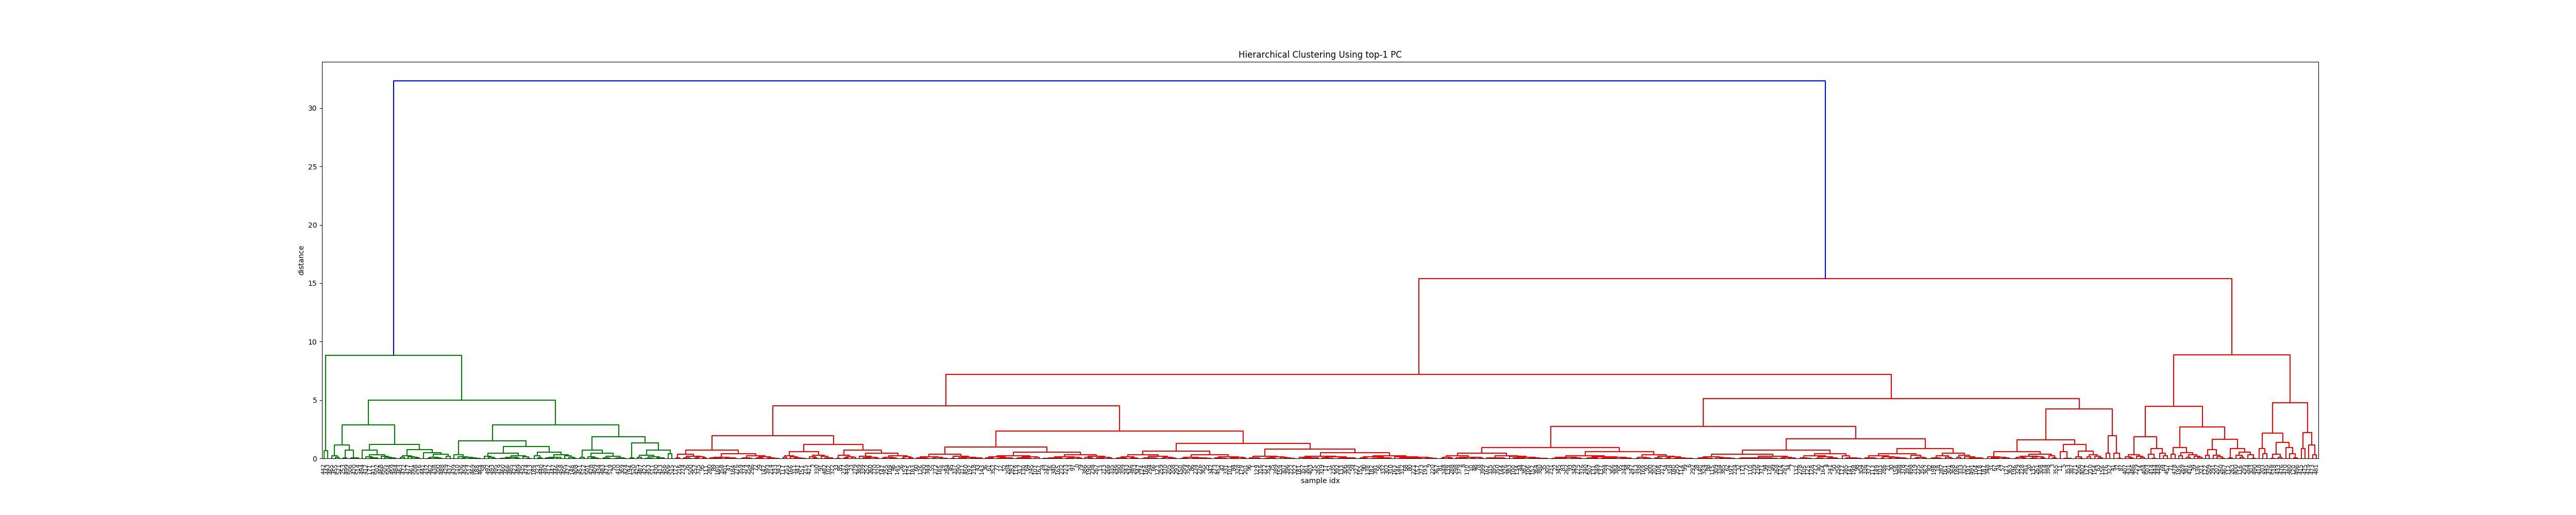
\includegraphics[scale=0.1]{../HClust-t1.png}
    \caption{Hierarchy Cluster with TOP1 Principle Component}
\end{figure}

可以直观的看到,降维后层次聚类明显迭代次数更少了。

利用该树进行二分类,评估分类准确率较比使用全部特征略有降低,但仍具有高置信度表现:
\begin{equation}
    Accuracy_{pca} = 90.80\%
\end{equation}

\section{PCA原理}

下面推导PCA数学原理,从两个角度进行推导。首先进行一些定义。

PCA的主要目的是在低维空间中寻找一组正交基$[u_1,\dots,u_M]$,使得数据在这组正交基形成的超平面上的投影方差最大。我们定义$U=[u_1,\dots,u_M]$,同时数据协方差定义为:
$$S=\frac{1}{N}\sum^N_{n=1}(x_n-\bar{x})(x_n-\bar{x})^T$$
\subsection{Maximum Variance}
在最大化方差思路中,我们目标是最大化:
\begin{equation}
    J=\frac{1}{N}||U^Tx_n-U^T\bar{x}||^2
\end{equation}

将其中的正交基展开可以有如下形式:
\begin{equation}
    J = \frac{1}{N}\sum^N_{n=1}\sum^M_{m=1}||u_m^Tx_n-u^T_m\bar{x}||^2 = \sum^M_{m=1}\frac{1}{N}\sum^N_{n=1}||u^T_mx_n-u^T_m\bar{x}||^2
\end{equation}

\begin{equation}
    \Rightarrow J = \sum^M_{m=1}u^T_mSu_m
\end{equation}

下面求解$J_m = $最大时对应的$u_m$满足什么条件,即转化为如下带约束的优化问题:
\begin{equation}
    \begin{aligned}
        argmin\ J_i &= u^T_i Su_i\\
        s.t.\quad u^T_iu_j&=\delta_{ij}
    \end{aligned}
\end{equation}

利用拉格朗日乘子法,构造函数:
\begin{equation}
    L = \sum^M_{m=1}u^T_mSu_m + \lambda_i(1-u^T_iu_i)
\end{equation}

求解$\frac{\partial L}{\partial u_i} = 0$,有:
\begin{equation}
    Su_i = \lambda_iu_i
\end{equation}

将上式结果带回目标中得到:
\begin{equation}
    J = \sum^M_{m=1}\lambda_m
\end{equation}

因此若想要目标$J$取得最大值,则需要选取协方差阵$S$前m个最大的特征值,故相应的转换矩阵中对应着前m个最大的特征值的特征向量。

\subsection{Minimun Error}
假设一组正交基构成M维空间,$\{u_i\},i\in D$,用$x_k$表示原D维空间中的k个点,$z_k$表示其在空间M上的投影,则
\begin{equation}
    z_k = \sum^M_{i=1}(u_i^Tx_k)u_i
\end{equation}

而为了最小化误差,我们的优化目标变成了;
\begin{equation}
    \begin{aligned}
    argmin &\sum^k_{i=1}||x_k-z_k||^2 \\
    s.t. &\quad u_i^Tu_j=\delta_{ij}
    \end{aligned}
\end{equation}

类似的利用拉格朗日乘子法,我们可以得到:
\begin{equation}
    argmin \ \sum_{i=M+1}^Du^T_iSu_i 
\end{equation}

而上式的约束恰恰与上一节中的推导相吻合,此处要求最小化剩余的维数,那么就应当使得前m维对应的特征值最大。
\section{EM \& GMM}
EM算法(最大期望)是一种寻找概率模型中寻找参数最大似然估计或最大后验估计的算法。主要有两个步骤:

\begin{itemize}
    \item[E步骤] $$Q(\Theta,\Theta^{(i-1)}) = E(logp(X,Y|\Theta)|X,\Theta^{(i-1)})$$
    \item[M步骤]$$\Theta^{(i)} = argmaxQ(\Theta,\Theta^{(i-1)}) $$
\end{itemize}
\subsection{EM of GMM}
首先该算法是一个迭代算法,因此初始值可以是一个估计,也可以是随机值$\Theta$,并开始迭代直至收敛。
混合高斯模型中需要有三个参数进行估计:
\begin{equation}
    p(x|\pi,\mu,\epsilon)=\sum^K_{k=1}\pi_kN(x|\mu_k,\epsilon_k)
\end{equation}
则利用EM算法估计这三个参数的步骤如下:
\begin{itemize}
    \item[E步骤]
$$Q(\Theta,\Theta^{i-1})=\sum^M_{k=1}\sum^N_{i=1}log(\pi_k)p(k|x_i,\Theta^{i-1})+\sum^M_{k=1}\sum^N_{i=1}log(p_k(x_i|\theta_k))p(k|x_i,\Theta^{i-1})$$ 
利用后验概率$P_i = p(k|x_i,\Theta^{i-1})$估计新的参数值:
    \item[M步骤]
$$\pi_k^i=\frac{1}{N}\sum^N_{i=1}P_i$$
$$\mu^i_k=\frac{\sum^N_{i=1}x_iP_i}{\sum^N_{i=1}P_i}$$
$$\epsilon^i_k=\frac{\sum^N_{i=1}P_i(x_i-\mu^i_k)(x_i-\mu^i_k)^T}{\sum^N_{i=1}P_i}$$ 
\end{itemize}

\subsection{K-means与GMM联系}
两种算法都是聚类迭代算法,但在每一次迭代中,K-means给出一个严格的分类,而GMM则给出模糊的分类(更倾向于是类别的概率)。从模型上,可以说K-means是一种特殊情况下的GMM模型,其中额外约束是其混合组分的协方差形如$\epsilon I$,其中$\epsilon \rightarrow 0$
\end{document}